%
% $Id$ 
%
% $LastChangedDate$ 
% 
% $LastChangedBy$
%

\documentclass[10pt]{report}
\usepackage{graphicx}
\usepackage{algorithm}
\usepackage{algorithmic}
\usepackage{setspace}                   
\onehalfspacing
% numbering down to subsubsection
\setcounter{secnumdepth}{3}

\title{CS6999 Web Data and Text Mining:\\Parallel Text Indexer Project Report}
\author{Damien DuBois\\Justin Kamerman 3335272\\Ramanpreet Singh 3395913}
\date{\today}

\begin{document}
\maketitle
% No chapter numbers
\renewcommand*\thesection{\arabic{section}}

%----------------------------------------
% Introduction
%----------------------------------------
\section{Introduction}
Fundamental to the real-world application of \textit{Information
  Retrieval} techniques is the ability to objectively measure the
quality of a particular algorithm or system and compare it to
others. Often, information retrieval algorithms lack an analytical
model that would allow one to make formal statements as to the
performance characteristics of a particular system. In addition, as with
machine learning and classification problems, using
a scalar value to represent the performance of a system as a whole is
misleading and does not account for the variety of operating
conditions under which the system may be expected to perform.

In measuring the performance of an information retrieval system, the
following factors constitute a set of operating conditions which
qualify the result:

\begin{itemize}
  \item Accuracy of the retrieval result with respect to the
    query. Common measures in this respect are \textit{Precision} and
    \textit{Recall}. Search techniques employing latent semantics of
    document collections are subtly more difficult to quantify, though
    measurable nonetheless.

    \item Speed with which queries are answered. This metric is a
      function of the number of search terms and the size of the
      corpus.

    \item Size of the document collection and, if not static, the rate
      at which new documents are being added and/or removed.
    

    \item The computational cost of the technique. Multiple
      activities may contribute to this aspect: searching, indexing,
      preprocessing, and post processing. It is important to consider
      whether the technique allows indices or intermediate
      approximations of the document collection to be altered
      incrementally or whether they must be regenerated to incorporate
      new documents. Also significant is whether the technique can be
      parallelized and thereby benefit from concurrency.

    \item The storage requirements of the technique. How do the
      storage requirements evolve with the size of the collection
      and/or degree of concurrency ?
\end{itemize}

To drive information retrieval research in one direction or another,
it would be useful to have a physical implementation
framework within which one could empirically explore the operating
characteristics of a particular algorithm and/or technique along the lines
described above. Such a system would allow researchers to investigate
how the system responds to variation in any one of these operating
parameters. The aim of this project is to create such an
information retrieval \textit{test-bed}.

The initial reference implementation of this information retrieval
test-bed is based on a simple \textit{inverted index} but has been
architected such that the specific algorithm could easily be changed
without significant rework. This paper presents a survey of existing
literature in support of our test-bed concept, as well as the specific
algorithms employed in the reference implementation. In
addition, a detailed architectural overview of the system is
presented, giving insight into how the system would be modified for
alternative algorithms. Lastly, an evaluation of our inverted index
reference implementation is conducted and the results analyzed.


%----------------------------------------
% Literature Review
%----------------------------------------
\section{Literature Review}
\label{sec:literaturereview}


\subsection{Indexing}
\textit{Information Retrieval} is a fast becoming the dominant form of
information access, overtaking traditional relational database style
searching \cite{RefWorks:109}. The basis of most document retrieval
systems is the \textit{term-document} incidence matrix. This matrix is
typically sparse and more efficiently represented as an
\textit{inverted-index} which maps terms to the parts of a document
where they occur. 

In order to construct an \textit{inverted index}, documents must be
scanned to determine \termit{term frequencies}. The Aho-Corasick
string matching algorithm\cite{RefWorks:103} is a simple and efficient
text scanning algorithm. The algorithm constructs a finite
state machine to scan for a given set of keywords. It is, in effect, a
reduced grammar regular expression parser of the type described in
\cite{RefWorks:111}. The algorithm is simple and efficient,
construction time being proportional to the sum of the length of the
keyword set, and the number of state transitions required to scan a
document is independent of the number of the size of the keyword
set. 


\subsection{Evaluation}
In the case of machine learning and classification systems, the
specification of a particular set of misclassification costs or false
and positive misclassification rates define a particular
\textit{operating point} of the system.

This concept applies equally to \textit{information retrieval} systems
whereby it is misleading to represent the operating characteristics of
a particular system with a scalar metric. In addition, the evaluation
of information retrieval systems suffers from the the inherent
subjectivity with respect to \textit{relevance}
\cite{RefWorks:72}. Non-scalar evaluation methods try to characterize
the performance of a system over a range of operating
conditions. Although this makes direct performance comparisons
ambiguous, we are more likely to be able to select the algorithm which
will perform best in the real world by applying domain expertise to
the results of a non-scalar evaluation \cite{RefWorks:32}.


\subsection{Parallelization}
Once an objective measure has been established, the performance of an
information retrieval system can be improved iteratively by making
various optimizations. These optimizations may take the form of
algorithm enhancements, implementation efficiencies, or
parallelization. 

Algorithm enhancements usually represent the forefront of research in
the field. Work to validate a new concept or algorithm is usually
performed in a very controlled environment and on relatively small
document collections. As the field matures, improvements are harder
fought and often involve increasingly complex algorithms and corpus
approximation methods into which it becomes more difficult to
\textit{fold-in} new documents. In addressing the considerable
computation cost of re-calculating \textit{Latent Semantic Indexing}
(LSI) \cite{RefWorks:102} approximations, \cite{RefWorks:101}
introduced new update methods which saw improved average precisions
but were forced to conclude that the improvements were at a
computational premium over previous methods. A semi-discrete matrix
decomposition for LSI, \textit{SDD}, performs as well as the original
SVD-based LSI method for equal query times and uses less storage
\cite{RefWorks:99}. The decomposition time of the new method, however,
is significantly larger than the original.

Enhancement of implementation efficiency in \cite{RefWorks:96} saw a
six-fold timing improvement in \textit{LSI} searches on large document
collections. The same study achieved nearly 180 times improvement
through the use of parallelization. The study made no algorithmic
improvements and the result is consistent with increased use of
parallelization by large commercial systems to cope with the ever
increasing bodies of data that must be processed.

\textit{Map-Reduce}, popularized by Google, is emerging as an
important programming model for large-scale data-parallel applications
such as web indexing \cite{RefWorks:113}. Fundamentally, Map-Reduce
breaks up a computation into smaller tasks which are made to run in
parallel on different physical machines. The \textit{map} and
\textit{reduce} phases are inspired by the functions of the same name
used in \textit{functional programming}. The model scales well to large
clusters mostly because of the decoupled nature of the tasks
themselves. An initial \textit{map} phase breaks the data into
  separate chunks and assigns them to a task. The \textit{reduce}
  phase assembles the results of the map tasks to produce the final
  result.

\textit{Hadoop} is an open source implementation of the MapReduce
model, developed mostly by Yahoo, and now maintained by the Apache
Software Foundation. Hadoop can be configured to automatically create
speculative copies of slow running map tasks
(stragglers). This facility is intended as a pre-emptive failure
recovery mechanism as well as a means of optimizing overall
throughput. The metrics used to identify stragglers as well as the
algorithm for determining the target node on which speculative copies
of a task should be launched, is examined in \cite{RefWorks:128}. The
paper introduces an alternative scheduling algorithm, \textit{LATE},
to address excessive task speculation issues with the native Hadoop
scheduler in a heterogeneous hardware environment. Experiments
comparing the native Hadoop scheduler, a non-speculative scheduling
strategy, and LATE were conducted using hosted virtual machines (VMs)
in the Amazon EC2 environment as well as a dedicated local
cluster. Variance in node performance was introduced by varying the
distribution of VMs across physical machines and also introducing
network and disk transfer loads. Results show speculative execution
(native Hadoop and LATE) outperforming non-speculative execution and
LATE outperforming native Hadoop in most cases.


%----------------------------------------
% Research Plan
%----------------------------------------
\section{Research Plan}
\label{sec:researchplan}
The primary goals of this research project is to construct an
information retrieval framework within which specific implementations
can be evaluated under various operating conditions. To initiate the
synthesis of this general framework, a reference implementation will
be built, based on the notion of a simple inverted index.

The software architecture of the reference implementation will be
carefully documented and follow established design patterns in order
to facilitate the future construction of alternative document search
schemes within the same framework. The framework will be designed to
be executed in a distributed deployment such that it may be used to
evaluate the effect of parallelization on a particular algorithm.

The performance of the reference implementation will be tested with
respect to the following operating parameters and compared to analytic
expectations:

\begin{itemize}
\item Number of index keywords
\item Number of documents in collection
\item Average size of documents
\end{itemize}

In addition, the reference implementation will be compared against a
na\"{i}ve implementation of the inverted indexer. The na\"{i}ve
implementation provided a baseline for further evaluation.


%----------------------------------------
% Design
%----------------------------------------
\section{Design}
\label{sec:design}
A black-box functional view of the indexing system is show in figure
\ref{fig:blackbox}. The system processes a continuous incoming flow of
documents and distribute them to parallel indexing threads running on
physically separate, heterogeneous nodes.  Document queries are performed
using an evolving search index. The operational balance is to
timeously index new additions to the corpus while servicing concurrent
search requests. A view as to how the components of the indexer system
are deployed is show in figure \ref{fig:deploymentmodel}.

As can be seen in figure \ref{fig:deploymentmodel}, the indexer
processes are symmetrical and deployed on multiple physical nodes. The
individual indexers do not interact directly with one another, making
for a simple deployment and operation model. The execution loop of
each indexer is as follows:

\begin{enumerate}
\item Initialize the indexer by retrieving a collection of index
  keywords and synonyms from a relational database. These keywords are
  used to construct a lexical parser which will be used to scan and
  index documents.
\item Retrieve a batch of unprocessed documents from a relational
  database. The document batch will be sized according to the physical
  capabilities of each node. In this implementation, this tuning task
  is a manual exercise but future enhancements may include an adaptive
  loading component.
\item Parse each document retrieved and construct an inverted index
  representing the batch. This \textit{delta} index, as we shall call
  it, is then used to augment the global index maintained in a
  relational database.
\item Repeat from step 2.
\end{enumerate}

As shown in figure \ref{fig:deploymentmodel}, the searcher component
can be executed from any node which has access to the relational
database housing the document index. The execution path of a single
search query wold be as follows:

\begin{enumerate}
  \item Canonize search terms based on keyword synonyms defined in the
    keyword store.
  \item Execute a boolean query against the inverted index.
  \item Return the list of corpus documents containing the
    intersection of the canons of the search terms.
\end{enumerate}

\begin{figure}
  \begin{center}
        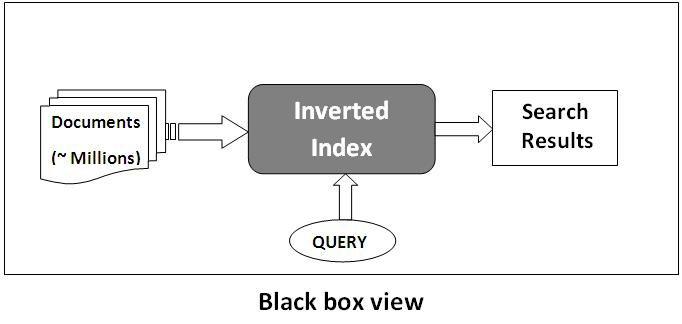
\includegraphics[width=\textwidth,height=!]{blackbox}
  \end{center}
  \caption{A black-box view of the indexer}
  \label{fig:blackbox}
\end{figure} 


\begin{figure}
  \begin{center}
        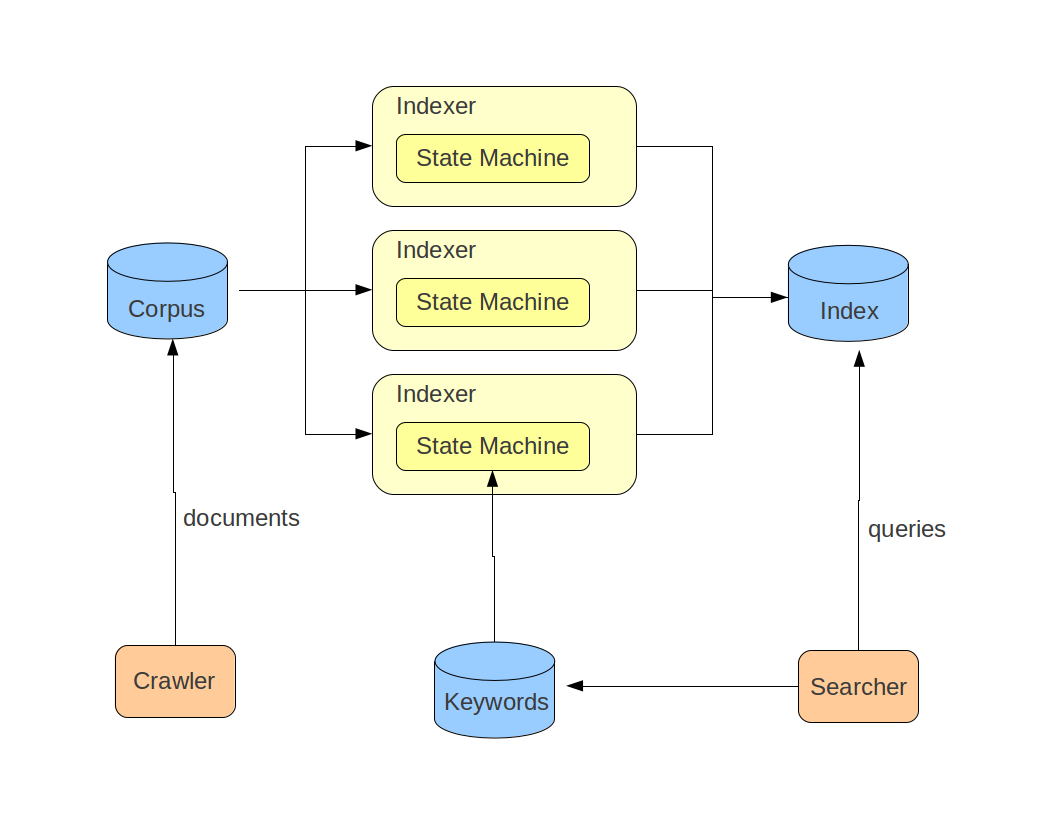
\includegraphics[width=\textwidth,height=!]{deploymentmodel}
  \end{center}
  \caption{Indexer deployment model}
  \label{fig:deploymentmodel}
\end{figure} 

A guiding architectural principal of the indexer design is to separate the implementation
into three logical layers:
\begin{itemize}
\item \textbf{Software Layer:} implements parsing, indexing and search
  algorithms.
\item \textbf{Data Access Layer:} implements an
  \textit{object-relational mapping}, insulating algorithm
  implementation from the persistence details. This layer implements
  classes which encapsulate persistent entities within the system.
\item \textbf{Database:} the persistent store for the document
  collection and inverted index.
\end{itemize}

The implementation classes and their relationships are represented in
a UML class diagram in figure \ref{fig:overallclassdiagram}. Figure
\ref{fig:overallsequencediagram} is a UML sequence diagram showing how
the layers interact at a high level.  The implementation of each of
these layers is described in more detail in section
\ref{sec:implementation}.

\begin{figure}
  \begin{center}
        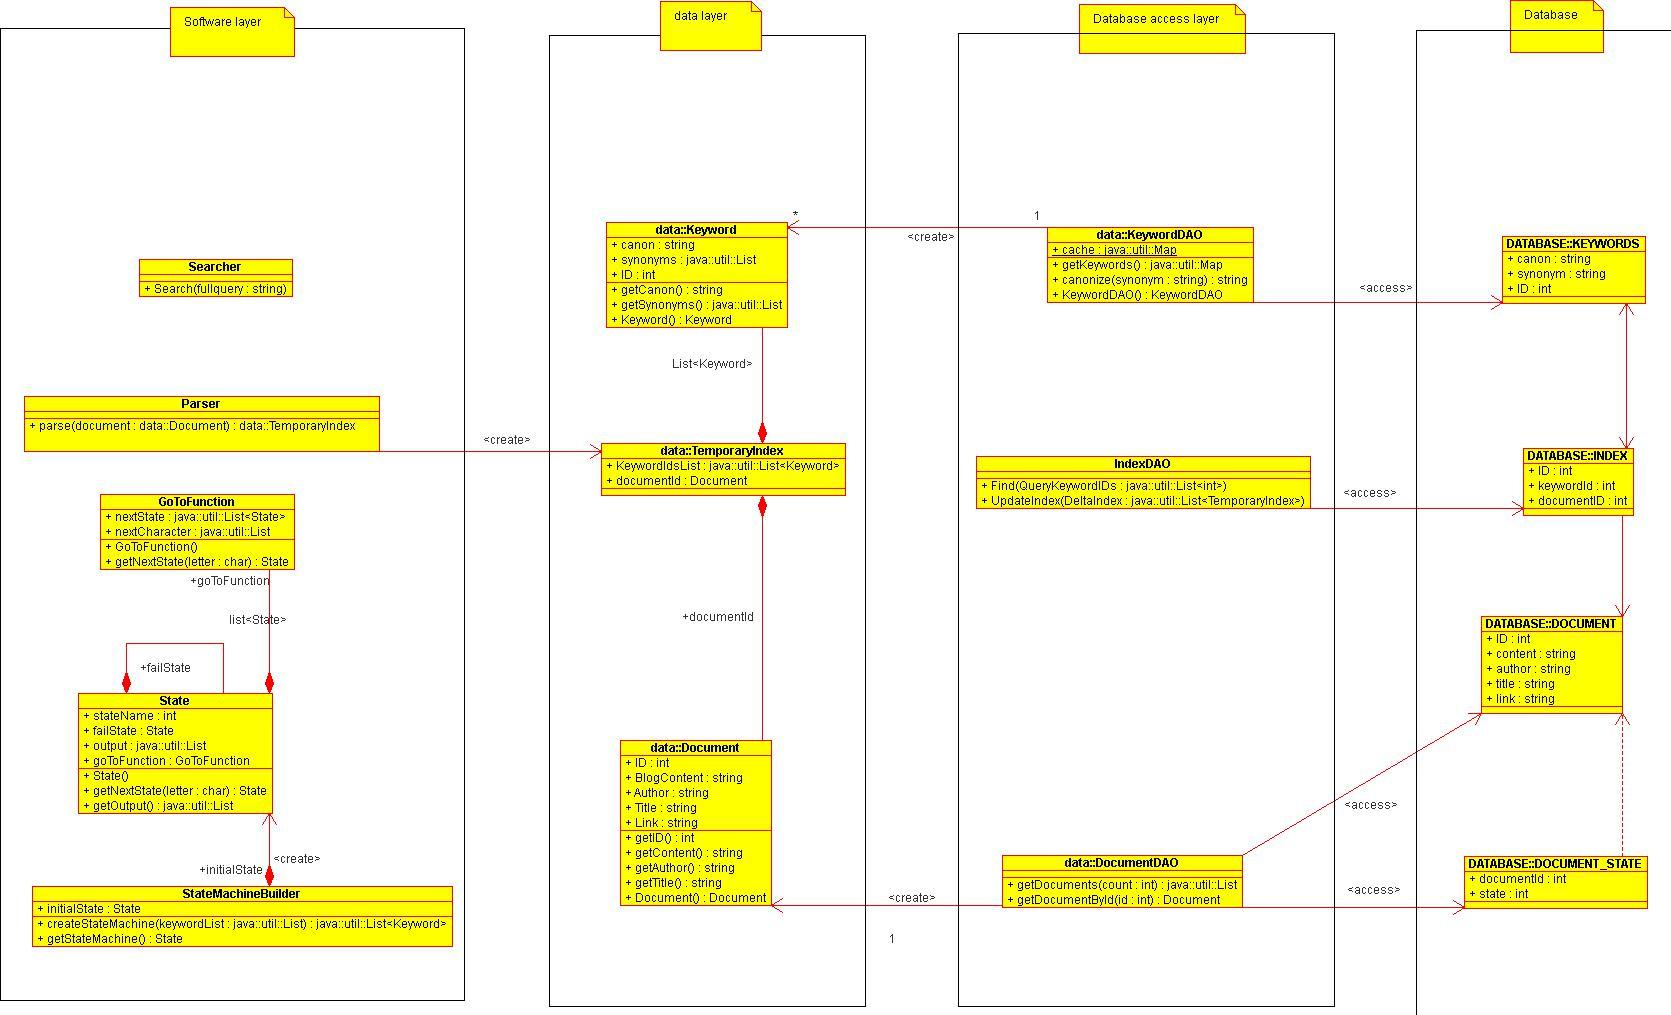
\includegraphics[angle=90,width=\textwidth,height=!]{overallclassdiagram}
  \end{center}
  \caption{Overall UML class diagram design}
  \label{fig:overallclassdiagram}
\end{figure} 

\begin{figure}
  \begin{center}
        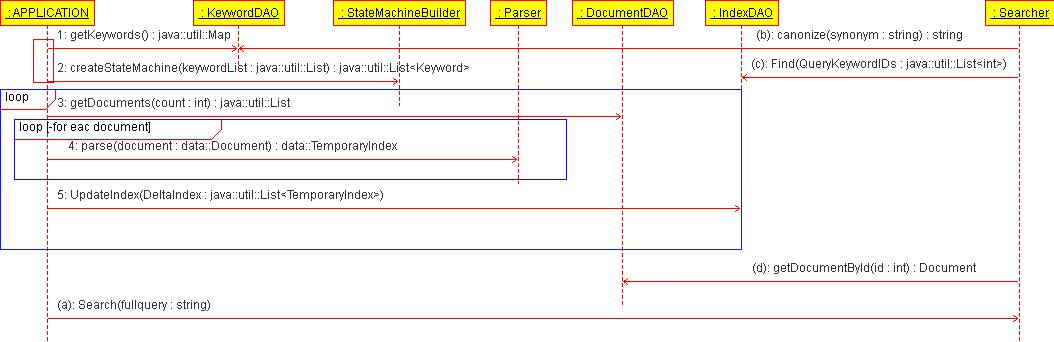
\includegraphics[width=\textwidth,height=!]{overallsequencediagram}
  \end{center}
  \caption{Overall UML sequence diagram design}
  \label{fig:overallsequencediagram}
\end{figure} 


%----------------------------------------
% Implementation 
%----------------------------------------
\section{Implementation}
\label{sec:implementation}
The individual worker processes of the indexer system are implemented as Java
programs. The programs make use of the following thirdparty libraries:

\begin{itemize}
  \item \textbf{DBPool:} a database connection pooling library, used
    to manage connections to relational databases.
  \item \textbf{Apache Commons Logging:} a generic logging API used by
    DBPool.
  \item \textbf{Apache Commons CLI:} a library for parsing command
    line arguments passed to Java programs.
  \item \textbf{MySQL JDBC driver:} the MySQL Java client driver.
\end{itemize}


The indexer system maintains an \textit{inverted index} of an evolving
corpus and services concurrent search requests against the index. The
current implementation is based on boolean retrieval methods described
in \cite{RefWorks:109}. An Aho-Corasick state machine
\cite{RefWorks:103} is used to scan documents for a predefined set of
keywords, and construct a term index for each document (delta
index). The term occurrences for each document are used to augment an
existing index of documents already processed. The document
collection, index, and keyword list are maintained in a single MySQL
database instance. It is through this database that the parallel
indexer instances are initialized and synchronized. This configuration
is operationally simple and easy to implement but the database has the
potential to become a throttle point as the system is scaled to larger
and more rapidly evolving document collections, and is required to
service a higher rate of queries. In order to scale the current
implementation to large document collections, a more efficient
mechanism would be required in this respect.

The following subsections detail the implementation of the
architectural layers identified in section \ref{sec:design}.

% Data Access Layer
\subsection{Data Access Layer}
\label{sec:dataaccesslayer}
Access to persistent storage is via objects of the data access
layer. Confining data access to a logical grouping of classes
insulates the other application components from changes in database
schema. The following subsections detail the individual data entities
handled by the data access later.


% Document
\subsubsection{Document}
\label{sec:document}
The \texttt{DocumentDAO} singleton class provides methods for retrieving
\texttt{Document} objects from the document database: 

\begin{itemize}
\item \texttt{List<Document> getDocuments (int count)}: retrieve a
  specified number of unprocessed documents from the database. The
  documents retrieved will be atomically marked as processed so that
  processing is not duplicated on other nodes. In this scheme, a
  document is considered \textit{processed} once retrieved from the
  database. This may cause problems from a fault recovery perspective
  if the processing node fails. A proposed enhancement to this scheme
  is to use an intermediate state, \textit{processing}, to indicate
  that the document has been retrieved and to update the state to
  \textit{processed} once processing is actually complete. For the
  initial implementation we will use the \textit{processed} state
  only.

\item \texttt{Document getDocumentById (int id)}: retrieve a specific
  document from the database, referenced by its ID. 

\item \texttt{int getID ()}: accessor method.
\item \texttt{String getContent ()}: accessor method.
\item \texttt{String getAuthor ()}: accessor method.
\item \texttt{String getTitle ()}: accessor method
\item \texttt{String getLink()}: accessor method.
\end{itemize}

The \texttt{Document} class encapsulates the BLOG database table, with the
addition of a state field that tracks whether a document has been
processed or not. Figures \ref{fig:documentclassdiagram} and
\ref{fig:documentsequencediagram} show class and sequence diagrams
respectively for non-trivial classes and methods involved in the
implementation of the Document data access layer. 

\begin{figure}
  \begin{center}
        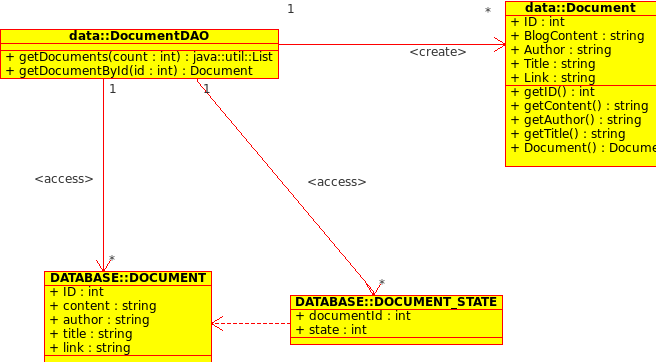
\includegraphics[width=\textwidth,height=!]{documentclassdiagram}
  \end{center}
  \caption{Document class diagram}
  \label{fig:documentclassdiagram}
\end{figure} 

\begin{figure}
  \begin{center}
        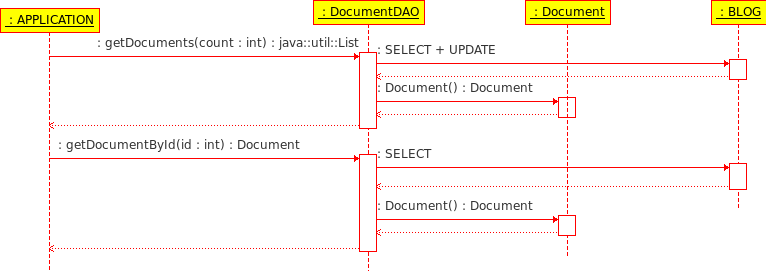
\includegraphics[width=\textwidth,height=!]{documentsequencediagram}
  \end{center}
  \caption{Document sequence diagram}
  \label{fig:documentsequencediagram}
\end{figure} 


% Keyword
\subsubsection{Keyword}
The \texttt{KeywordDAO} singleton class provides methods for
retrieving \texttt{Keyword} objects from the document
database. Because the keyword set is relatively static and accessed
often, the full set of keywords will be loaded from the database and
cached when the class initializes. The class also provides methods for
converting search terms to their canonical form.

\begin{itemize}
\item \texttt{List<String> getKeywords ()}: this method
  will returns a list of all \texttt{Keyword} objects defined in the
  keyword database. 

\item \texttt{List<Integer> canonize (String query)}: return the list
  of IDs corresponding to a comma-separated list of query terms.

\item \texttt{Keyword getKeywordById (int id)}: return the
  \texttt{Keyword} object with the given identifier.
\end{itemize}

The \texttt{Keyword} field encapsulates a canonical search term and a
list of its synonyms. Figures \ref{fig:keywordclassdiagram} and
\ref{fig:keywordsequencediagram} show UML class and sequence diagrams
respectively for non-trivial classes and methods involved in the
implementation of the Keyword data access layer. 

\begin{figure}
  \begin{center}
        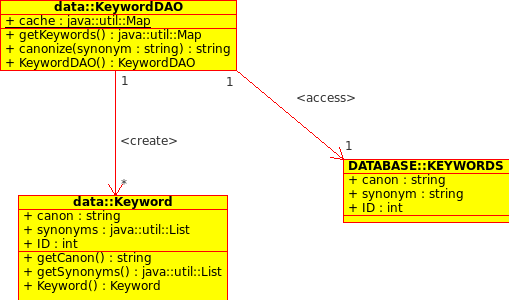
\includegraphics[width=\textwidth,height=!]{keywordclassdiagram}
  \end{center}
  \caption{Keyword class diagram}
  \label{fig:keywordclassdiagram}
\end{figure} 

\begin{figure}
  \begin{center}
        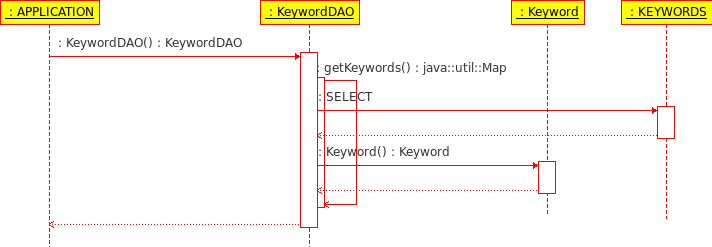
\includegraphics[width=\textwidth,height=!]{keywordsequencediagram}
  \end{center}
  \caption{Keyword sequence diagram}
  \label{fig:keywordsequencediagram}
\end{figure} 


% Index
\subsubsection{Index}
The \texttt{IndexDAO} class provides methods for updating and
searching the inverted index table stored in the database. There are
two methods defined in this class: 

\begin{itemize}
\item \texttt{void UpdateIndex (List<TempIndex> input)}: this method
  takes input of type List<TempIndex> (Note: Temporary index is a user
  defined data class, which contains Document ID and List of <keyword
  ids> as its attributes) and generates an SQL query which updates the
  INDEX table in the Database. 

\item \texttt{List<Integer> Find (List<Integer> QueryKeywordIds)}:
  this method takes a list of \texttt{Integers} (which corresponds to
  mapped \texttt{String} query into keyword ids) as input and searches
  the INDEX table in DB to find all the document ids which are common
  between for the given query keywords. 
\end{itemize}

 Figures \ref{fig:indexclassdiagram} and
 \ref{fig:indexsequencediagram} show UML class and sequence
 diagrams respectively for classes and methods involved in the
 implementation of the Index data access layer.

\begin{figure}
  \begin{center}
        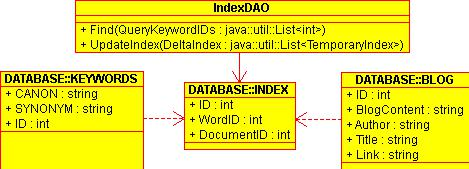
\includegraphics[width=\textwidth,height=!]{indexclassdiagram}
  \end{center}
  \caption{Index class diagram}
  \label{fig:indexclassdiagram}
\end{figure} 

\begin{figure}
  \begin{center}
        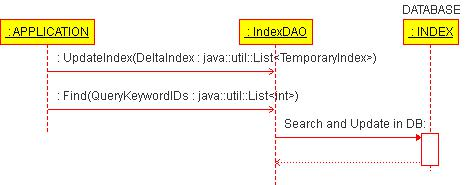
\includegraphics[width=\textwidth,height=!]{indexsequencediagram}
  \end{center}
  \caption{Index sequence diagram}
  \label{fig:indexsequencediagram}
\end{figure} 


% Software Layer
\subsection{Software Layer}

% Searcher
\subsubsection{Searcher}
This class is designed to perform searches for a query entered by the
user. It contains a method named \texttt{search ()} which is responsible for
finding all the documents which contained all query keywords.

\begin{itemize}
\item \texttt{List<Document> search (String)}: given a comma-separated
  list of search terms, returns the list of documents in which the
  canonical form of all search terms appear together. This method
  First calls \texttt{List<int> KeywordDAO.canonize (String)}, to map
  string query keywords into corresponding list of keyword IDs.  Note:
  We are assuming that the query will be formed with the set of
  keywords, which will be a subset of the global keyword set, with
  which the parsing state machine is constructed.

  Then it calls \texttt{List<Integer> IndexDAO.find
    (List<querykeywordIDs>)}, which will searches in INDEX DB for a
  list of Common DOC\_IDs corresponding to given query keywords.

  In the end, it calls \texttt{List<Document>
    DocumentDAO.getDocumentById (DOC\_ID)}. This will map DOC\_ID into
  a \texttt{Document} from the BLOG table in the database. 
\end{itemize}
 
Figures \ref{fig:searcherclassdiagram} and
\ref{fig:searchersequencediagram} show UML class and sequence
diagrams respectively for classes and methods involved in the
implementation of the \texttt{Searcher} class.


\begin{figure}
  \begin{center}
        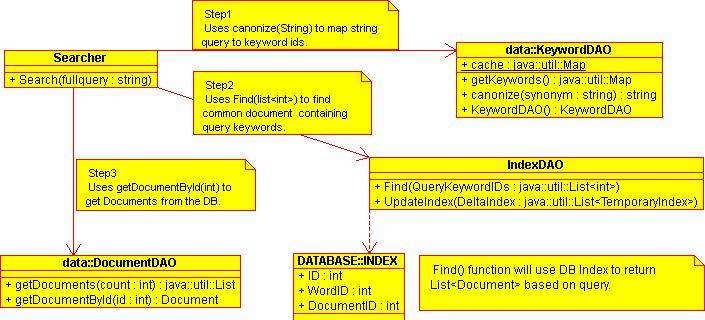
\includegraphics[width=\textwidth,height=!]{searcherclassdiagram}
  \end{center}
  \caption{Searcher class diagram}
  \label{fig:searcherclassdiagram}
\end{figure} 

\begin{figure}
  \begin{center}
        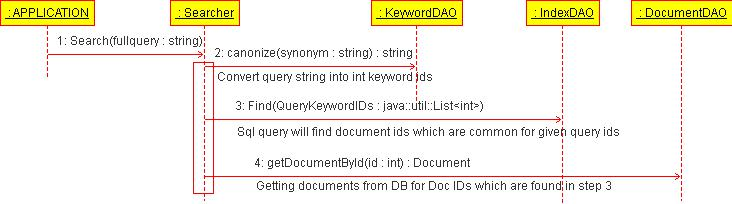
\includegraphics[width=\textwidth,height=!]{searchersequencediagram}
  \end{center}
  \caption{Searcher sequence diagram}
  \label{fig:searchersequencediagram}
\end{figure} 


% State Machine
\subsubsection{State Machine}
This class is designed to build the state machine from the list of
keywords returned by the \texttt{KeywordDAO.getKeywords()} method. This class has a static
attribute \texttt{initialState} that is the first state of the state machine
built by the function \texttt{createStateMachine} (initializes with the value
null). The first state gives us the whole state machine thanks to the
architecture of a state. Once the state machine is built, the function
\texttt{getStateMachine} is used to access the initial state stored in the
class.

Figures \ref{fig:statemachineclassdiagram} and
\ref{fig:statemachinesequencediagram} show UML class and sequence
diagrams respectively for classes and methods involved in the
implementation of the \texttt{StateMachineBuilder}.

\begin{figure}
  \begin{center}
        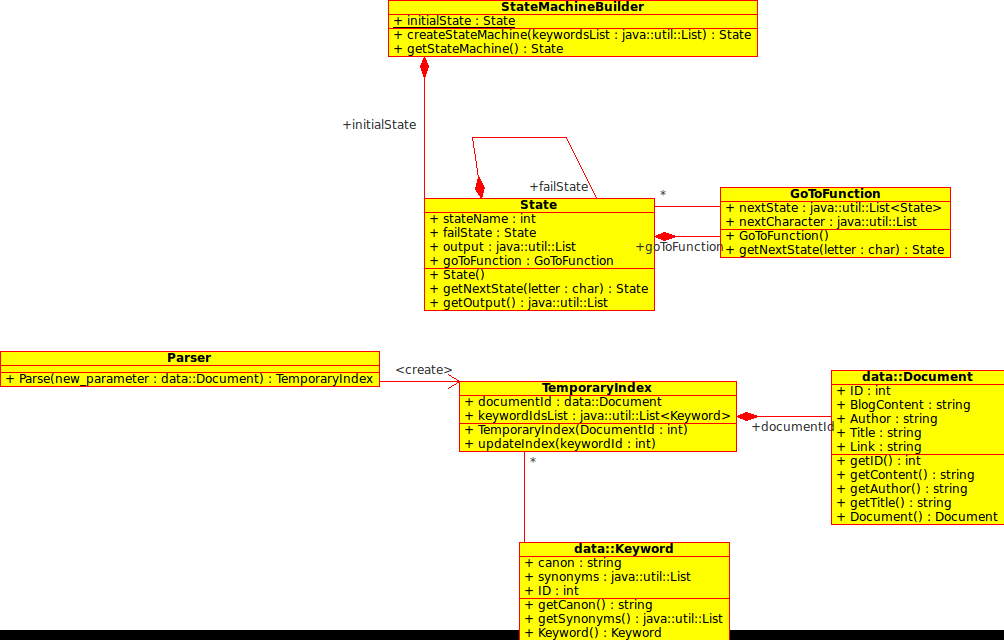
\includegraphics[width=\textwidth,height=!]{statemachineclassdiagram}
  \end{center}
  \caption{State machine class diagram}
  \label{fig:statemachineclassdiagram}
\end{figure} 

\begin{figure}
  \begin{center}
        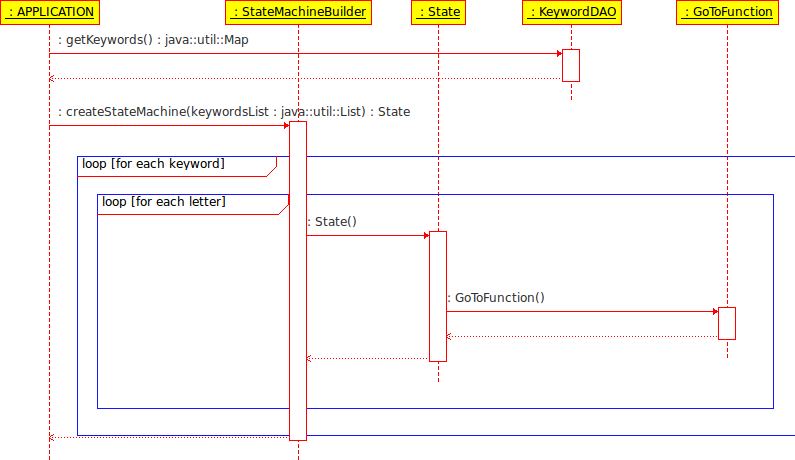
\includegraphics[width=\textwidth,height=!]{statemachinesequencediagram}
  \end{center}
  \caption{State machine sequence diagram}
  \label{fig:statemachinesequencediagram}
\end{figure} 


% Parser
\subsubsection{Parser}
The \texttt{Parser} implements the document parsing algorithm within
the state machine. By default, it uses the state machine contained
in the static attribute of \texttt{StateMachineBuilder}. To parse a
document we need to call the \texttt{parse ()} function inside this
class, passing it the \texttt{Document} class encapsulating the actual
text we want to parse. This class returns a \texttt{TemporaryIndex}
object which encapsulates a reference to the document parsed and the
keywords found to occur within the document.

Figures \ref{fig:parserclassdiagram} and
\ref{fig:parsersequencediagram} show UML class and sequence
diagrams respectively for classes and methods involved in the
implementation of the \texttt{Parser}.

\begin{figure}[h!]
  \begin{center}
        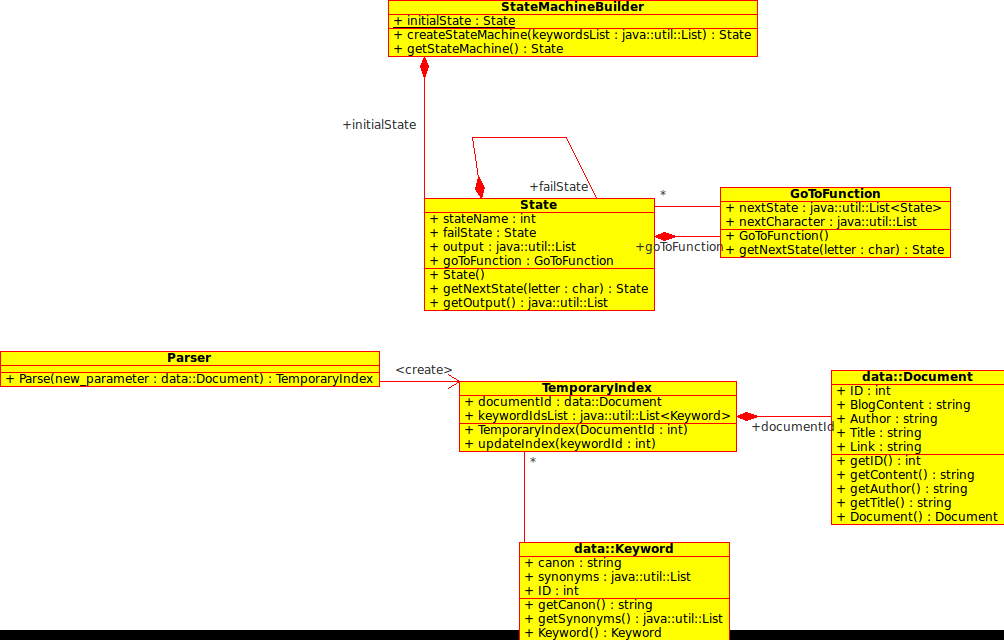
\includegraphics[width=\textwidth,height=!]{parserclassdiagram}
  \end{center}
  \caption{Parser class diagram}
  \label{fig:parserclassdiagram}
\end{figure} 

\begin{figure}[h!]
  \begin{center}
        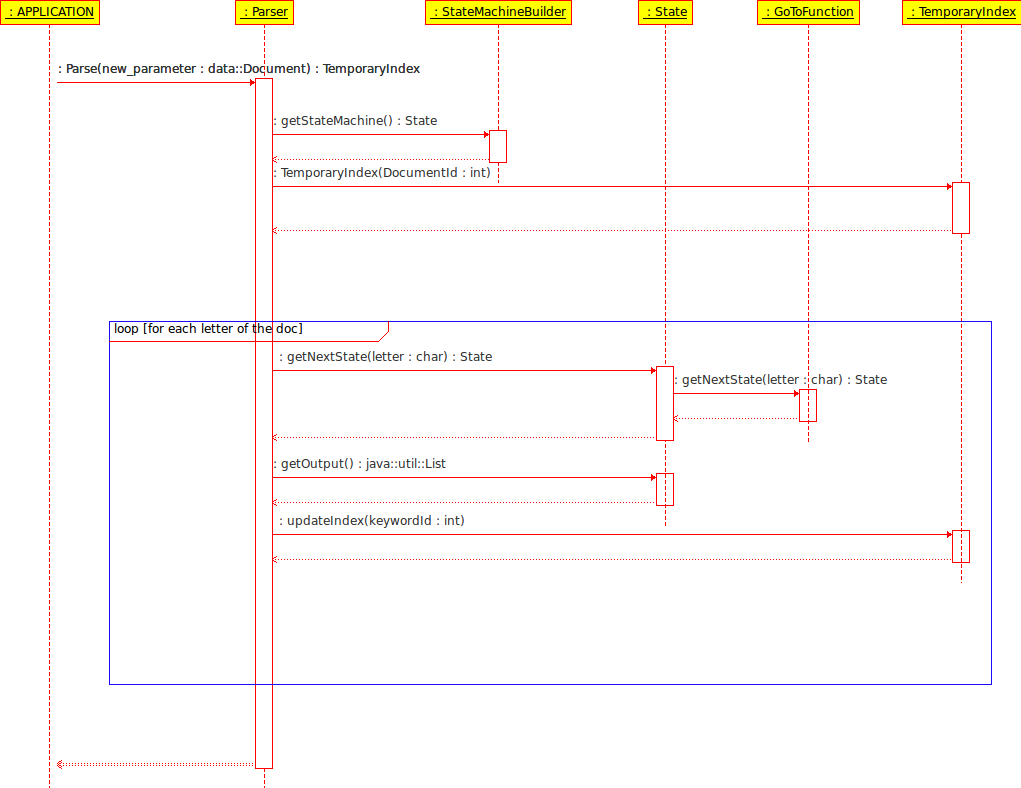
\includegraphics[width=\textwidth,height=!]{parsersequencediagram}
  \end{center}
  \caption{Parser sequence diagram}
  \label{fig:parsersequencediagram}
\end{figure} 


%----------------------------------------
% Experiment Results
%----------------------------------------
\section{Experiment Results}
\label{sec:experimentresults}
The primary goal of this project is to be able to reduce the time
to build a document index. As our system is building the inverted index by
parsing all documents of the collection, we can expect the
time complexity of the task to be proportional to the sum total of
characters in the collection. As a result, changing the  
number of documents or the average size of each document should
have a big impact in our time complexity. In addition, our
implementation will incur the cost of building the Aho-Corasick state
machines used to scan the documents. We can expect the time to build a
state machine to be proportional to the sum of the size of the
keywords. 

Finally we will do a time comparison between our indexer
implementation and a na\"{i}ve implementation. All the time
complexities tests are done on a single computer and it is important
to understand that all these processes can be parallelized. In section
\ref{parallelization} we install our indexer on multiple computers and
explore the performance gain of running parallel instances
simultaneously.


All tests were run on a single Intel Core 2 Duo 2GHz processor, 1GB
RAM, running a 64-bit Linux 2.6.35 SMP kernel. The Java Virtual
Machine used was version 1.6.0-24. The database used was MySQL,
running on the same node as the indexer.


%----------------------------------------
% Number of Keywords
%----------------------------------------
\subsection{Number of Keywords}
To be able to study the impact of different number of keywords, we
built a keywords database with 10,000 most popular English
words \cite{wordlist}. All the experiments in this
part are done with 50,000 posts randomly downloaded from the Internet. The
idea is to get a good distribution of documents with respect to length
and content. The experiment shown here consist of building the index
for different numbers of keywords from the 10,000 keyword database and
explore the time and space complexity for the building of the state
machine and the building of the index using the state machine.


\subsubsection{Time Complexity}
\begin{itemize}
\item \textbf{State Machine Construction:}
  The time taken to construct the Aho-Corasick state machine was
  measured for different numbers of keywords. The results of this test
  is shown in figure \ref{fig:numkeywordstimecomplexbuildsm} and construction time
  can easily be considered linear with respect to the number of
  keywords. This is consistent with \cite{RefWorks:103} which proves
  that the state machine construction algorithm is linearly
  proportional to the sum of the lengths of the keywords used to
  construct the state machine.

  \begin{figure}[h]
    \begin{center}
      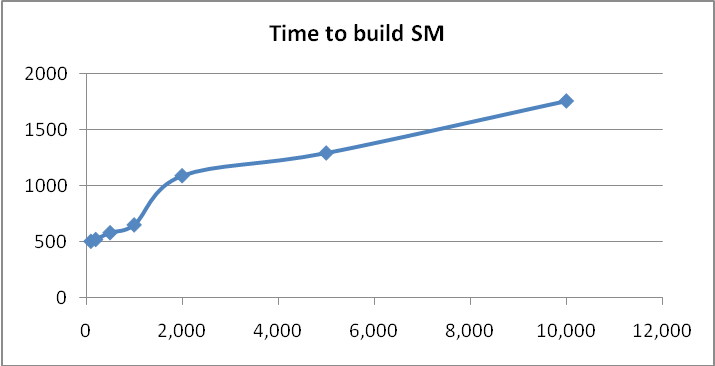
\includegraphics[width=\textwidth,height=!]{numkeywordstimecomplexbuildsm}
    \end{center}
    \caption{Time to build Aho-Corasick state machine as a function of
      the number of keywords. Time taken is shown in milliseconds on the
      y-axis and the number of keywords on the x-axis}
    \label{fig:numkeywordstimecomplexbuildsm}
  \end{figure} 
  
\item \textbf{Index Construction:} 
  The time taken for a state machines to build an inverted index of our
  corpus was measured. The test was repeated using state machines
  constructed with a varying number of keywords and the results plotted
  in figure \ref{fig:numkeywordstimecomplexbuildindex}. According to
  \cite{RefWorks:103} which proves that the number of state transitions
  involved in processing an input string is independent of the number of
  keywords used to construct the state machine, we would not expect the
  time complexity to increase with the size of the keyword set. However,
  as can be seen in \ref{fig:numkeywordstimecomplexbuildindex}, the time
  to build the index increases logarithmically with the number of
  keywords. This is likely due to the fact that as the number of keywords
  increases, so does the size of the index and the number of database
  interacts required to store and update the index.

  \begin{figure}[h]
    \begin{center}
      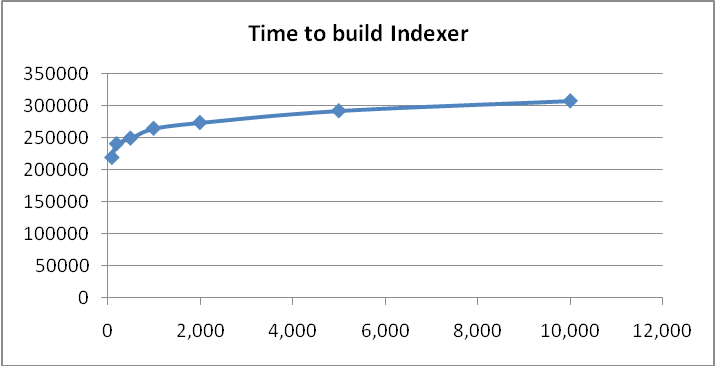
\includegraphics[width=\textwidth,height=!]{numkeywordstimecomplexbuildindex}
    \end{center}
    \caption{Time to build the inverted index as a function of the
      number of keywords. Time taken is shown in milliseconds on the
      y-axis and the number of keywords on the x-axis}
    \label{fig:numkeywordstimecomplexbuildindex}
  \end{figure} 

\end{itemize}


\subsubsection{Space Complexity}
As we would have expected it, the space used by the index in the
database is proportional to the number of words we are using. It also
means that our words have the same probability at the beginning or at
the end of our 12,000 word dictionary. This result is reflected in
figure \ref{fig:numkeywordsspacecomplexbuildindex}.

\begin{figure}
  \begin{center}
    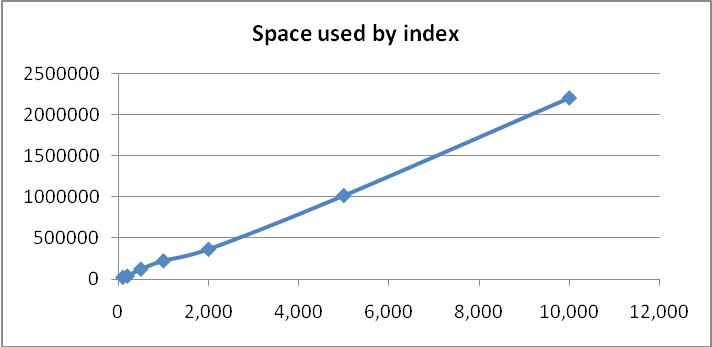
\includegraphics[width=\textwidth,height=!]{numkeywordsspacecomplexbuildindex}
  \end{center}
    \caption{Size of index as a function of the number of
      keywords. The number of database rows used to store the index is
      shown on the y-axis and the number of keywords on the x-axis} 
    \label{fig:numkeywordsspacecomplexbuildindex}
\end{figure} 


%----------------------------------------
% Size of Corpus
%----------------------------------------
\subsection{Size of Corpus}
To be able to study the impact of different number of Posts, we built
a posts database with 400,000 posts randomly downloaded from
the Internet. Then the keywords used to build the index are simply the
first 5,000 from the previous keywords database. 

The experiment shown here consist on building the index for different
number of Posts and explore the time and space complexity for the
building of the state machine and the building of the index once the
state machine is built. We can expect that the time to build the State
machine won’t change with the number of posts and the time to build
the index will increase almost linearly with the number of posts.  


\subsubsection{Time Complexity}
As we were expecting, the time to build the index with the state
machine strategy is linear with respect to the number of post, as
depicted in figure \ref{fig:corpsizetimecomplexbuildindex}. However, to be able
to perform this experiment we had to run the indexer program with
batches of 10,000 posts due to Java heap space problems. As a result, the state
machine is rebuilt every 10,000 posts.  

\begin{figure}[h!]
  \begin{center}
    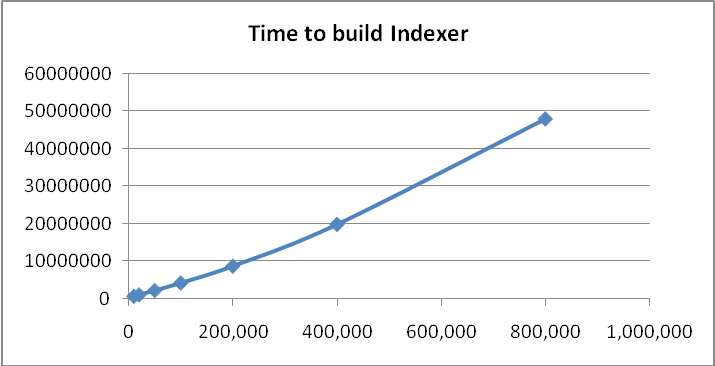
\includegraphics[width=\textwidth,height=!]{corpsizetimecomplexbuildindex}
  \end{center}
    \caption{Time to build the inverted index as a function of the
      size of the corpus. Time taken is shown in milliseconds on the
      y-axis and the number of documents in the collection on the
      x-axis} 
    \label{fig:corpsizetimecomplexbuildindex}
\end{figure} 


\subsubsection{Space Complexity}
As expected, the space used to store the index in the database is
proportional to the size of the corpus. This result is shown in figure
\ref{fig:corpsizespacecomplexbuildindex}.

\begin{figure}[h!]
  \begin{center}
    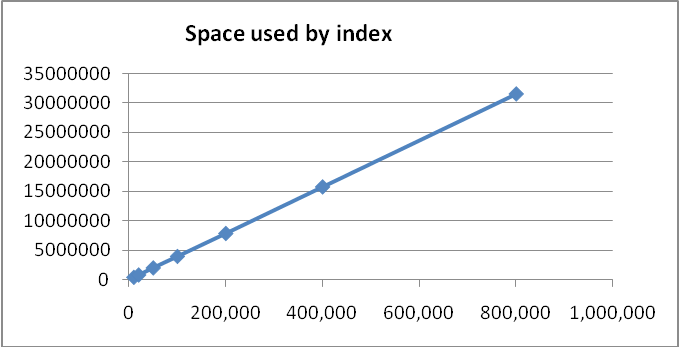
\includegraphics[width=\textwidth,height=!]{corpsizespacecomplexbuildindex}
  \end{center}
    \caption{Size of index as a function of the size of the
      corpus. The number of database rows used to store the index is
      shown on the y-axis and the number of documents in the
      collection on the x-axis} 
    \label{fig:corpsizespacecomplexbuildindex}
\end{figure}


%----------------------------------------
% Document Size
%----------------------------------------
\subsection{Document Size} 
As we have seen before, the time to build the index is almost
proportional with the number of post. Theoretically this time should
be proportional to the total length of all posts. Let’s focus on this
aspect and study the impact of the length of the post on the time to
build the state machine. To do that we built a 5,000 posts database
with posts that are all composed of 20,000 characters. Then, we ran
our system on different length of substring of these posts.  


\subsubsection{Time Complexity}
\begin{itemize}
\item \textbf{State Machine Construction:} 
  As expected, state machine construction time
  does not depend on the length of the documents. Nonetheless it is
  interesting to compare figures \ref{fig:docsizetimecomplexbuildsm}
  and \ref{fig:docsizetimecomplexbuildindex}, showing the construction
  times for the state machine and inverted index relative to the
  average document size. The comparison shows that state machine
  construction time is several orders of magnitude smaller than index
  construction and negligible by comparison. Our state machine is
  built in 770 ms on average for 1000 keywords with a standard
  deviation of 18ms. 

  \begin{figure}[h!]
    \begin{center}
      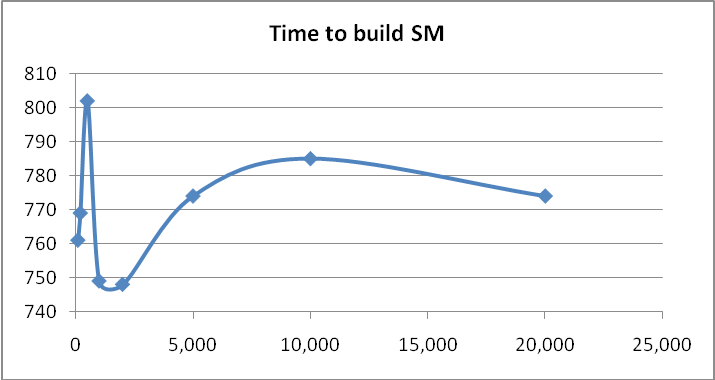
\includegraphics[width=\textwidth,height=!]{docsizetimecomplexbuildsm}
    \end{center}
    \caption{Time to build Aho-Corasick state machine as a function of
      the average document size. Time taken is shown in milliseconds on the
      y-axis and the average document size in characters on the x-axis}
    \label{fig:docsizetimecomplexbuildsm}
  \end{figure} 

\item \textbf{Index Construction:} 
  As expected the time to build the indexer is almost linear with
  respect to the average document size. This relationship is shown in
  figure \ref{fig:docsizetimecomplexbuildindex}.

  \begin{figure}[h!]
    \begin{center}
      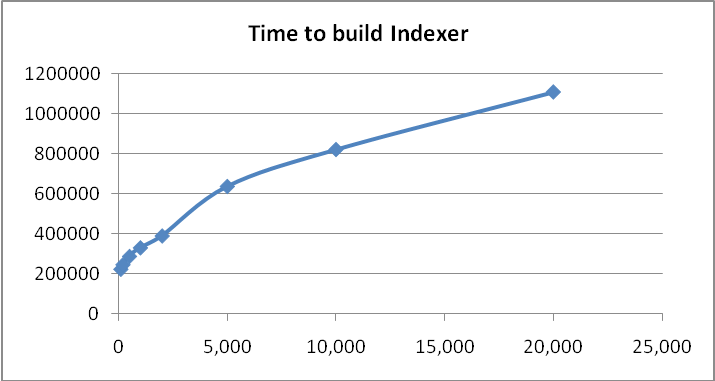
\includegraphics[width=\textwidth,height=!]{docsizetimecomplexbuildindex}
    \end{center}
    \caption{Time to build an inverted index as a function of the
      average document size. Time taken is shown in milliseconds on the
      y-axis and the average document size in characters on the x-axis} 
    \label{fig:docsizetimecomplexbuildindex}
  \end{figure} 

\end{itemize}


\subsubsection{Space Complexity}
Here we are studying the number of records in our index database as a
function of the average document size. As expected, the larger the documents
the more records created to represent the index. However, this is not linear
since if a word occurs many times in the same post we just save it
once in the database. This relationship is shown in figure
\ref{fig:docsizespacecomplexbuildindex}. 

\begin{figure}[h!]
  \begin{center}
    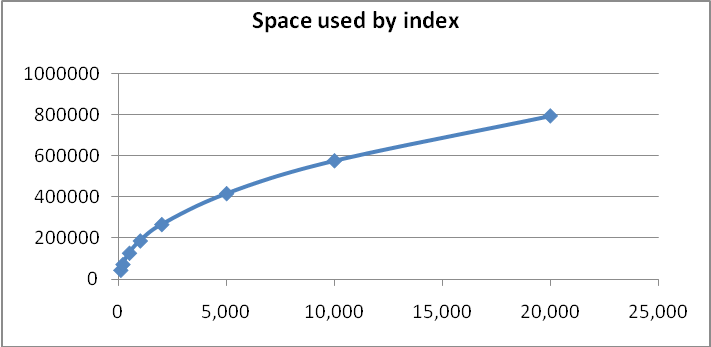
\includegraphics[width=\textwidth,height=!]{docsizespacecomplexbuildindex}
  \end{center}
  \caption{Size of index as a function of the average document
    size. The number of database rows used to store the index is
      shown on the y-axis and the average document size in characters
      on the x-axis}  
  \label{fig:docsizespacecomplexbuildindex}
\end{figure} 


%----------------------------------------
% Comparison with Naive Index Builder
%----------------------------------------
\subsection{Comparison with Na\"{i}ve Index Builder}
This part focuses on the improvement that our system with respect to
time complexity in comparison with a na\"{i}ve index builder. The na\"{i}ve
indexer builder has the same input as our system i.e. a list of
keywords and a list of documents, and the same output i.e. an inverted
index corresponding to the keywords and documents. Algorithm
\ref{alg:invertedindex} is used in principal for both implementations.


\begin{algorithm}
\caption{Build inverted index}
\label{alg:invertedindex}
\begin{algorithmic}
  \FORALL{$keyword$}
  \STATE Build a vector $v$
  \FORALL {$document$}
  \IF {$keyword$ \epsilon \; $document$}
  \STATE Add the row (keyword.id, document.id) into $v$
  \ENDFOR
  \STATE Save $v$ into the database
  \ENDFOR
\end{algorithmic}
\end{algorithm}

As we can see this algorithm has a complexity that directly depends on
the number of keywords $n$, the number of document $m$, and the length
of document since we have to check in each document for each
keyword. Moreover, we decided to limit, as much as possible, the
accesses to the database since it is really time consuming in
Java. That’s why we do one access to the database for each keywords
and not for each document. In the state machine we do as much accesses
to the database as the number of document (in the worst case meaning
we find at least one keyword per document). In the following
subsections we compare the results for this algorithm with our system
results for different number of keywords and posts.


\subsubsection{Complexity Analysis}
For the na\"{i}ve algorithm described above, the theoretical worst
case time complexity relationship is shown in equation
\ref{eqn:timecomplexworstcase}.  

\begin{equation}
\label{eqn:timecomplexworstcase}
Time \propto keyNum * ( docNum * maxLength + conn)
\end{equation}

where \(keyNum\) is the number of keywords, \(docNum\) is the number
of documents, \(maxLength\) is the maximum document length, and
\(conn\) is the time taken to create a connection to the database. For
the state machine algorithm the theoretical complexity relationship is
given by 
equation \ref{eqn:timecomplexsm}.

\begin{equation}
\label{eqn:timecomplexsm}
Time \propto docNum * ( maxLength + conn)
\end{equation}


\subsubsection{Document Size}
For this experiment we fixed the number of keywords to 1,000 and the
number of documents to 5,000 and we ran our code on a database
composed of document of different length. The experiment results are
shown in figure \ref{fig:naivedocumentsize}.

\begin{figure}[h!]
  \begin{center}
    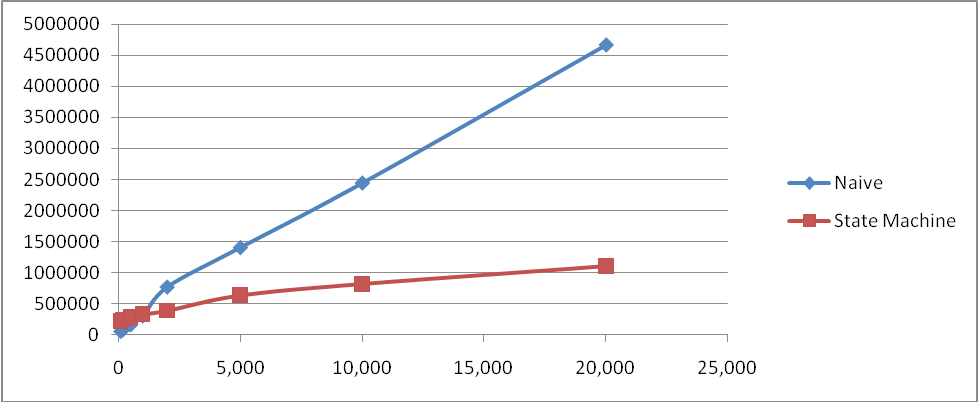
\includegraphics[width=\textwidth,height=!]{naivedocumentsize}
  \end{center}
  \caption{Time to build an inverted index as a function of the
      average document size. Time taken is shown in miliseconds on the
      y-axis and the average document size in characters on the x-axis}
  \label{fig:naivedocumentsize}
\end{figure} 


As expected, the curves for both our indexer and the naive indexer are
almost linear since for the naive implementation:

\[Time \propto (keyNum * docNum) * maxLength + conn * keyNum\]

and for our Aho-Corasick state machine method: 

\[Time \propto docNum * maxLength + conn * docNum\]

We can observe that for a small length of document naive method is
faster since \(keyNum\) is smaller than \(docNum\). For \(docLength = 1300\)
our indexer is far more efficient. To see this effect more clearly,
experiment results are plotted on a logarithmic scale in figure
\ref{fig:naivedocumentsizelog}.

\begin{figure}[h!]
  \begin{center}
    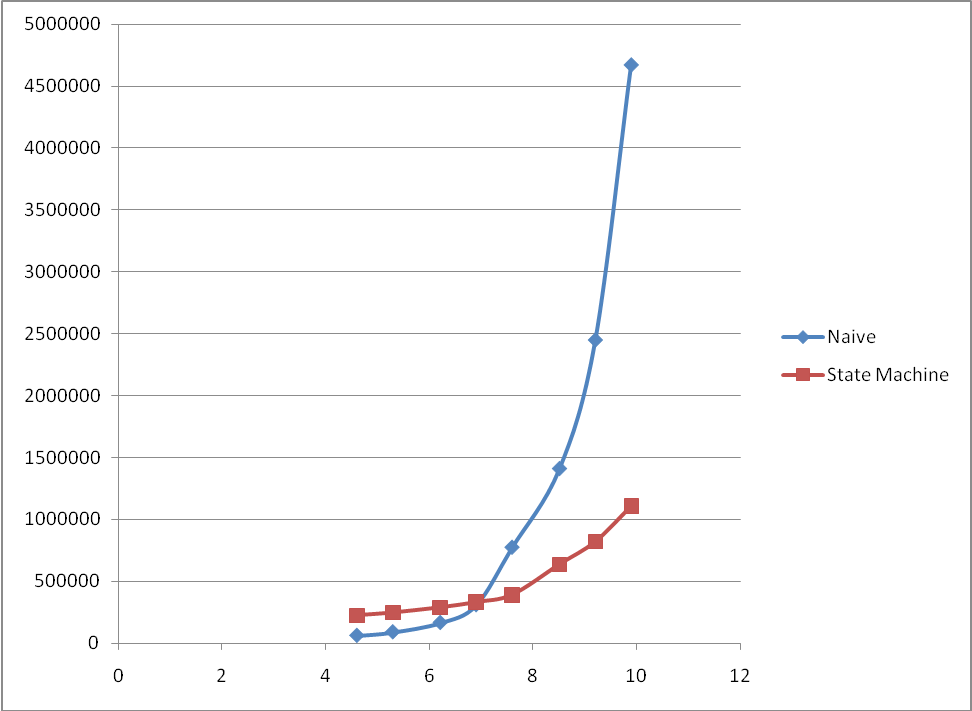
\includegraphics[width=\textwidth,height=!]{naivedocumentsizelog}
  \end{center}
  \caption{Time to build an inverted index as a function of the
      average document size. Time taken is shown in milliseconds on the
      y-axis and the average document size in characters on the
      logarithmic x-axis}
  \label{fig:naivedocumentsizelog}
\end{figure} 


\subsubsection{Number of Keywords}
As expected, the two implementations exhibit a linear response to the
number of keywords used. In the na\"{i}ve implemementation:

\[Time \propto (keyNum * maxLength) * docNum + conn * keyNum\]

and in our Aho-Corasick state machine method: 

\[Time \propto (maxLength + conn) * docNum \]

However, we would have expected the state machine method not to depend
on the number of keyword. The reason why it’s not the case is because
when we don’t have any keywords in a document, we don’t access the
database. Knowing that the database access is very time consuming,
increasing the number of keyword increases the probability of finding a
keyword into each document and so increase the time complexity.  

The experiment results are shown in figure \ref{fig:naivenumkeywords}
and on a logarithmic scale in figure \ref{fig:naivenumkeywordslog}.

\begin{figure}[p]
  \begin{center}
    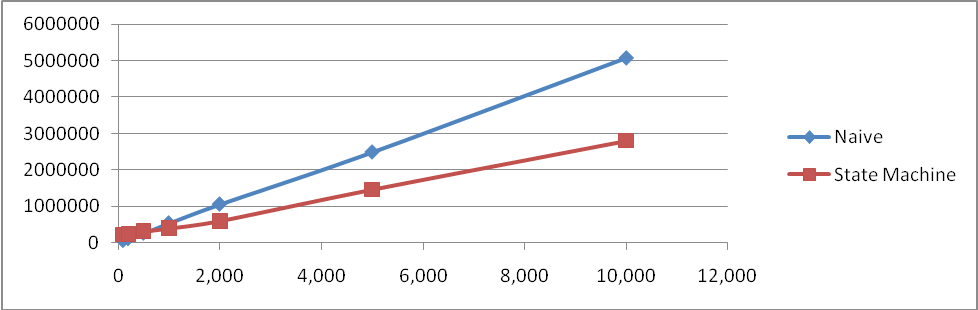
\includegraphics[width=\textwidth,height=!]{naivenumkeywords}
  \end{center}
  \caption{Time to build an inverted index as a function of the
      number of keywords. Time taken is shown in milliseconds on the
      y-axis and the number of keywords on the x-axis}
  \label{fig:naivenumkeywords}
\end{figure} 


\begin{figure}[p]
  \begin{center}
    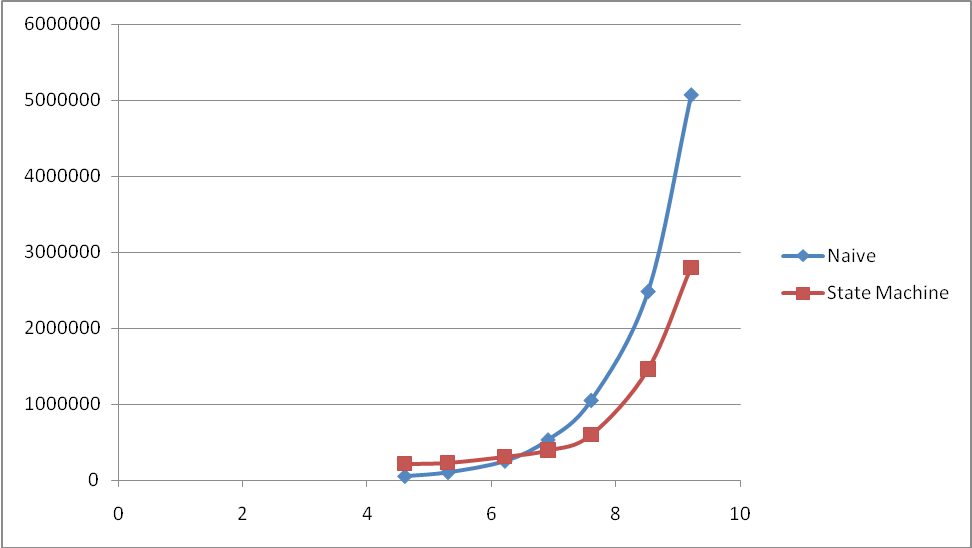
\includegraphics[width=\textwidth,height=!]{naivenumkeywordslog}
  \end{center}
  \caption{Time to build an inverted index as a function of the
      number of keywords. Time taken is shown in milliseconds on the
      y-axis and the number of keywords on the logarithmic x-axis}
  \label{fig:naivenumkeywordslog}
\end{figure} 


\subsubsection{Size of Corpus}
As expected, the time complexity is linearly related to the number of
documents being indexed. The experiment results are shown in figure
\ref{fig:naivesizecorpus} and on a logarithmic scale in figure
\ref{fig:naivesizecorpuslog}. For the na\"{i}ve implementation:

\[Time \propto (docNum * maxLenght + conn) * keyNum\]
 
and in our Aho-Corasick state machine method: 

\[Time \propto docNum * maxLenght + conn * docNum\]


\begin{figure}[p]
  \begin{center}
    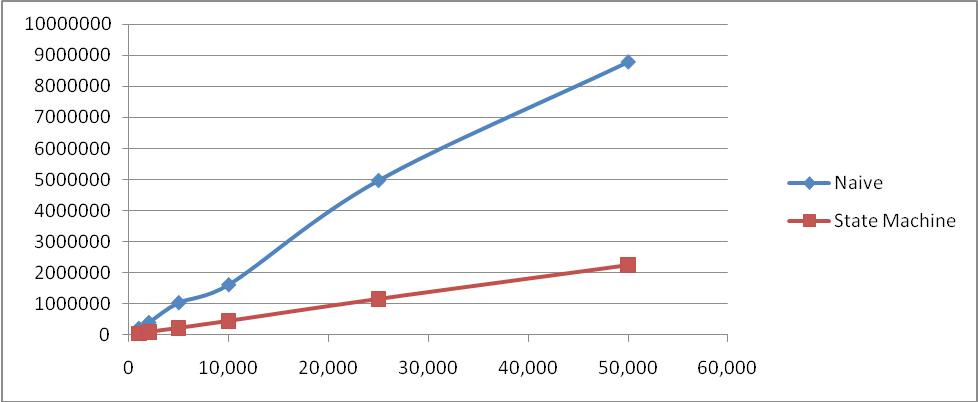
\includegraphics[width=\textwidth,height=!]{naivesizecorpus}
  \end{center}
  \caption{Time to build an inverted index as a function of the
      number of documents being indexed. Time taken is shown in
      milliseconds on the y-axis and the number of documents on the
      x-axis} 
  \label{fig:naivesizecorpus}
\end{figure} 


\begin{figure}[p]
  \begin{center}
    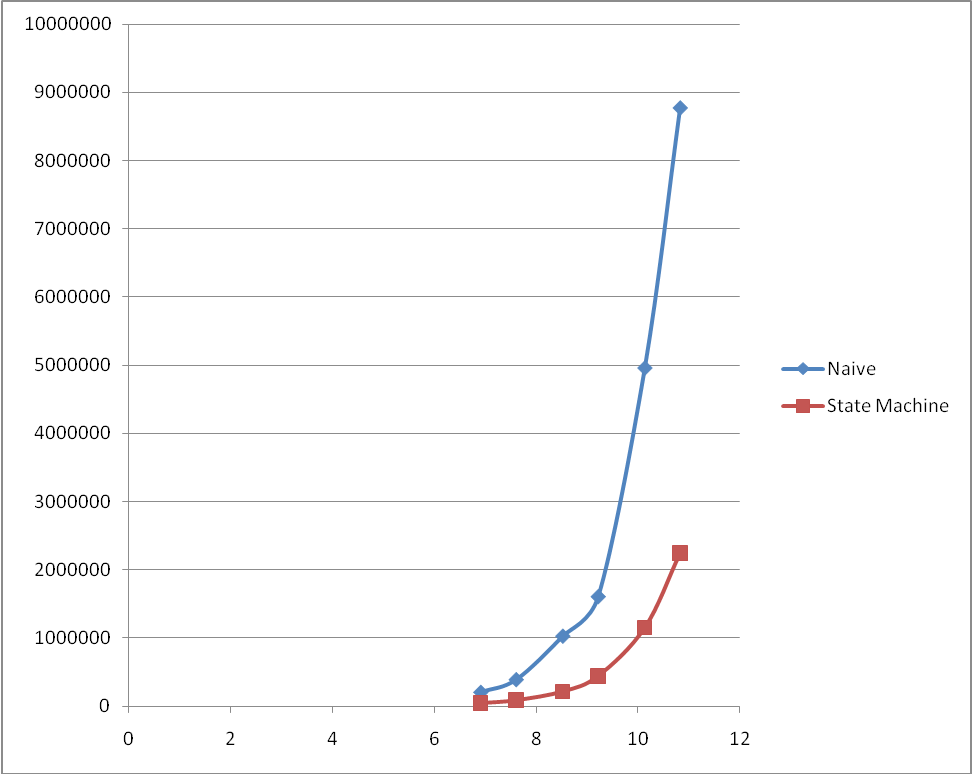
\includegraphics[width=\textwidth,height=!]{naivesizecorpuslog}
  \end{center}
  \caption{Time to build an inverted index as a function of the
      number of documents being indexed. Time taken is shown in
      milliseconds on the y-axis and the number of documents on the
      logarithmic x-axis} 
  \label{fig:naivesizecorpuslog}
\end{figure} 


%----------------------------------------
% Parallelization
%----------------------------------------
\subsection{Parallelization}
\label{parallelization}

\begin{figure}[p]
  \begin{center}
    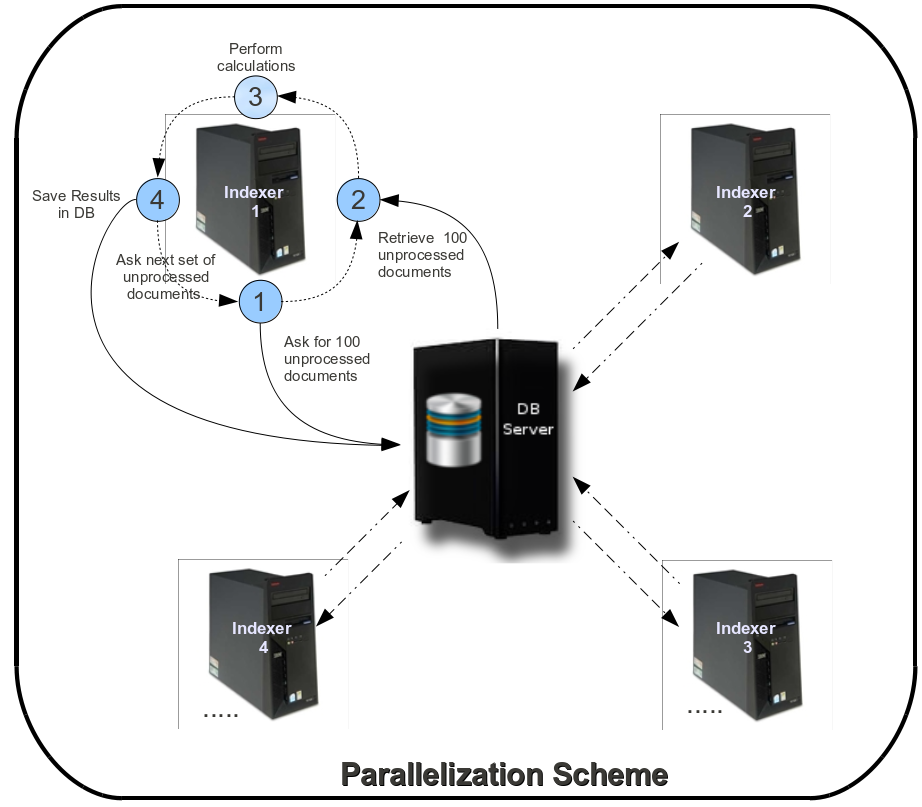
\includegraphics[width=\textwidth,height=!]{paralleldeploymentmodel}
  \end{center}
  \caption{Deployment model of parallel indexer} 
  \label{fig:paralleldeploymentmodel}
\end{figure} 


%----------------------------------------
% Conclusions
%----------------------------------------
\section{Conclusions}
\label{sec:conclusions}
The experimental results tend to prove what we could expect from
theory. Our system is faster than the na\"{i}ve indexer with respect
to the number of keywords being indexed, size of the document
collection, and average document size. In particular, our indexer
implementation performs relatively well with respect to the number of
documents being indexed. Moreover, as soon as we are dealing with a number of
keywords that can be representative of real-world needs, the state
machine implementation proves also to be significantly faster than the
naive indexer. 

One of the primary goals of this research project was to leverage the
effect of parallelization in reducing the time to index a document
collection. Due to time constraints, this was not done but the
resulting implementation lays a strong foundation for further research
in this area. Other avenues of interest include, but are not limited
to:

\begin{itemize}
  \item Compare the Aho-Corasick state machine indexer implementation
    to less na\"{i}ve indexer implementations.
    
    \item Use compression techniques to our algorithm in order to
      reduce the index size in the database.

    \item Study the time performance improvements possible deploying
      the Aho-Corasick state machine indexer within a commercial
      \textit{MapReduce} framework such as \textit{Hadoop}.
\end{itemize}



%----------------------------------------
% Bibliography
%----------------------------------------
% changes default name Bibliography to References
\renewcommand\bibname{References}
\bibliography{bibliography}
\bibliographystyle{IEEEannot}


%--------------------------------------------------
\end{document}
